%  Verwendete Plattform /Software (Installationshinweise, Versionen)
% Schnittstellenbeschreibung des Web Services (WSDL/WADL/Swagger, …​)
% Umsetzung, Technologien, Sicherheitskonzepte, API

\section{Technologien}

\subsection{Übersicht verwendeter Technologien, Software  \newline und Formate}


Die Anwendung besteht aus verteilten Micro-Services, die mit Hilfe von Docker containerisiert wurden. Jeder Micro-Service basiert auf einem Spring-Boot Container und nutzt den Netflix-Stack (Eureka und Zuul), um sich bei einer Service-Registry zu registrieren. Die nun auffindbaren Services können gegenseitig miteinander kommunizieren und ein API-Gateway (Zuul) delegiert Requests an die entsprechenden Services.
Die Micro-Services bieten jeweils eine eigene REST-API an, die mit Hilfe des Web-Frontends konsumiert werden kann. 
Die in der Anwendung genutzten Technologien aus Tabelle \ref{tab:Technologien}  sind in Abbildung \ref{fig:TechStack} noch einmal schematisch zugeordnet. 
Eine Zuordnung der Technologien zur Architektur erfolgt in Abbildung \ref{fig:ArchitekturTech}

Anmerkung: Die Andoid-App wurde nicht im Rahmen der Lehrveranstaltung fertig gestellt und ist somit noch ausstehend. Da sie aber für eine spätere Nutzung angedacht ist und sie ebenfalls über die REST-Schnittstelle kommuniziert wurde sie im Entwurf berücksichtigt. 

% Tabelle 
\renewcommand{\arraystretch}{1.3} % Abstände zwischen den Spalten 
\begin{table}[H] 
	% \small
	\centering
	\caption{Technologien}
	\begin{tabularx}{\textwidth}{l|c|X}
		\textbf{Name} & \textbf{Version} & \textbf{Verwendung} \\
		\hline
		Java & JDK 1.8.0 & Verwendete Programmiersprache \\
		Maven & 3.1.0  & Build-Management-Tool \\
		Spring Boot & 2.0.2 & Java Framework für Backends \\
		MySQL & 5.7.0 & Relationale Datenbank \\
		Netflix Zuul & 1.3.1 & Edge Service für dynamisches Routen, \newline Monitoring und Sicherheit  \\
		Netflix Eureka & 1.9.2 &  Service-Registry   \\
		JSON & - & Datenaustauschformat \\
		REST & - & Programmierparadigma für Webservices \\
		React & 16.1.1 & JavaScript Bibliothek für User Interfaces  \\
		single-spa & 2.6.0 & JavaScript Framework für Front-End Microservices \\
		OpenAPI  (Swagger) & 3.0 & Definition der REST-Schnittstelle; Automatisches Generieren von Java-Interfaces  \\
		Postman & 6.5.3 & API Development Environment, \newline Testen der API \\
		Docker & 18.09.0 & Umgebung für Container, Deployment \\
	\end{tabularx}
	\label{tab:Technologien}
\end{table}

\begin{figure}[H]
	\hspace{-1.5cm}
	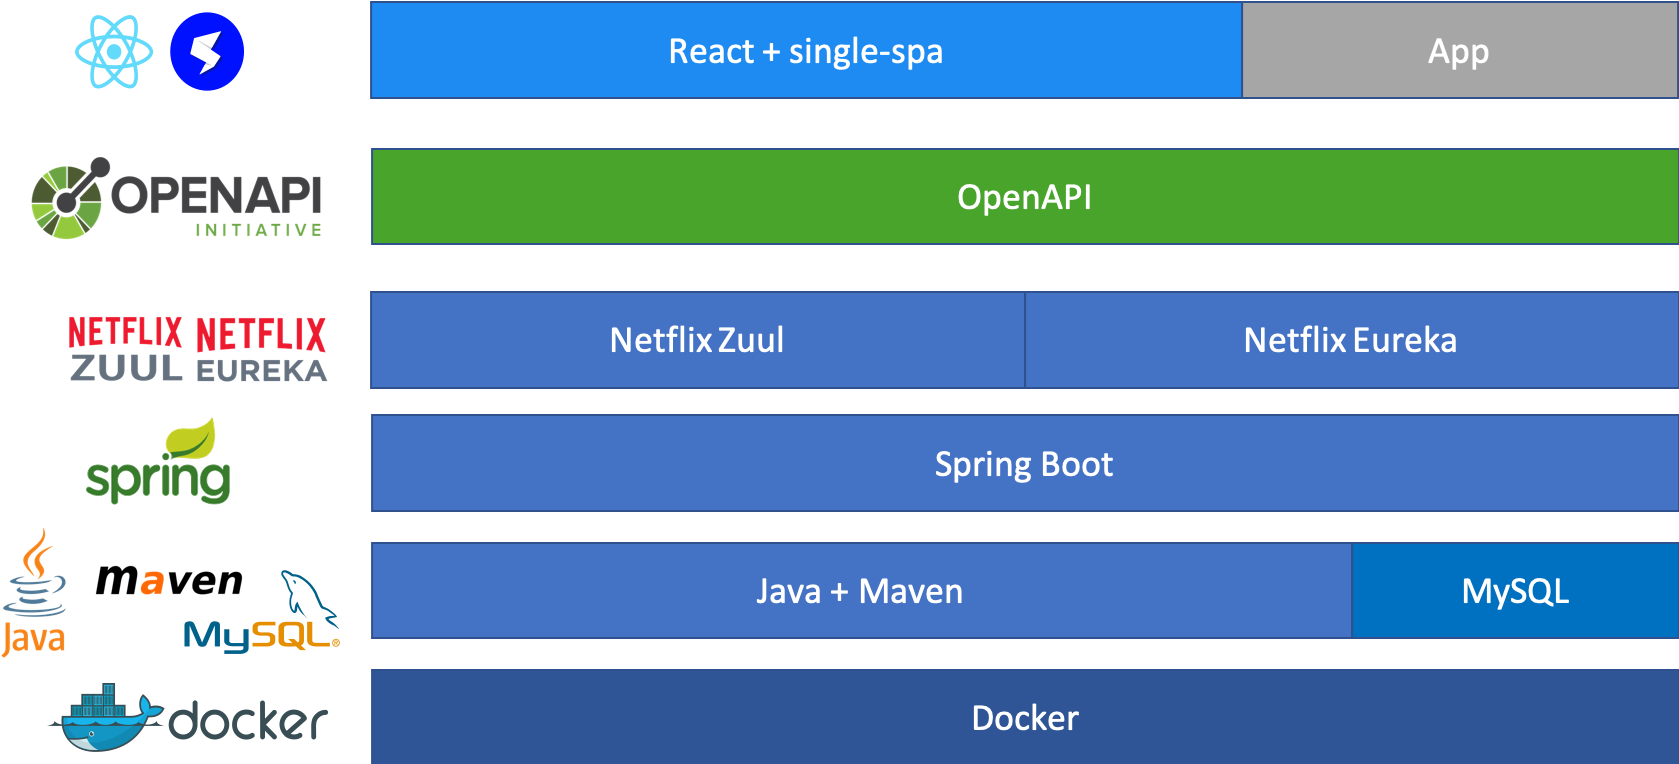
\includegraphics[width=1.15\linewidth]{technology_stack.png}
	\caption{Technologie Stack}
	\label{fig:TechStack}
\end{figure}

\subsection{Architektur}

%Beschriebender Text?

\begin{figure}[H]
	\hspace{-1.5cm}
	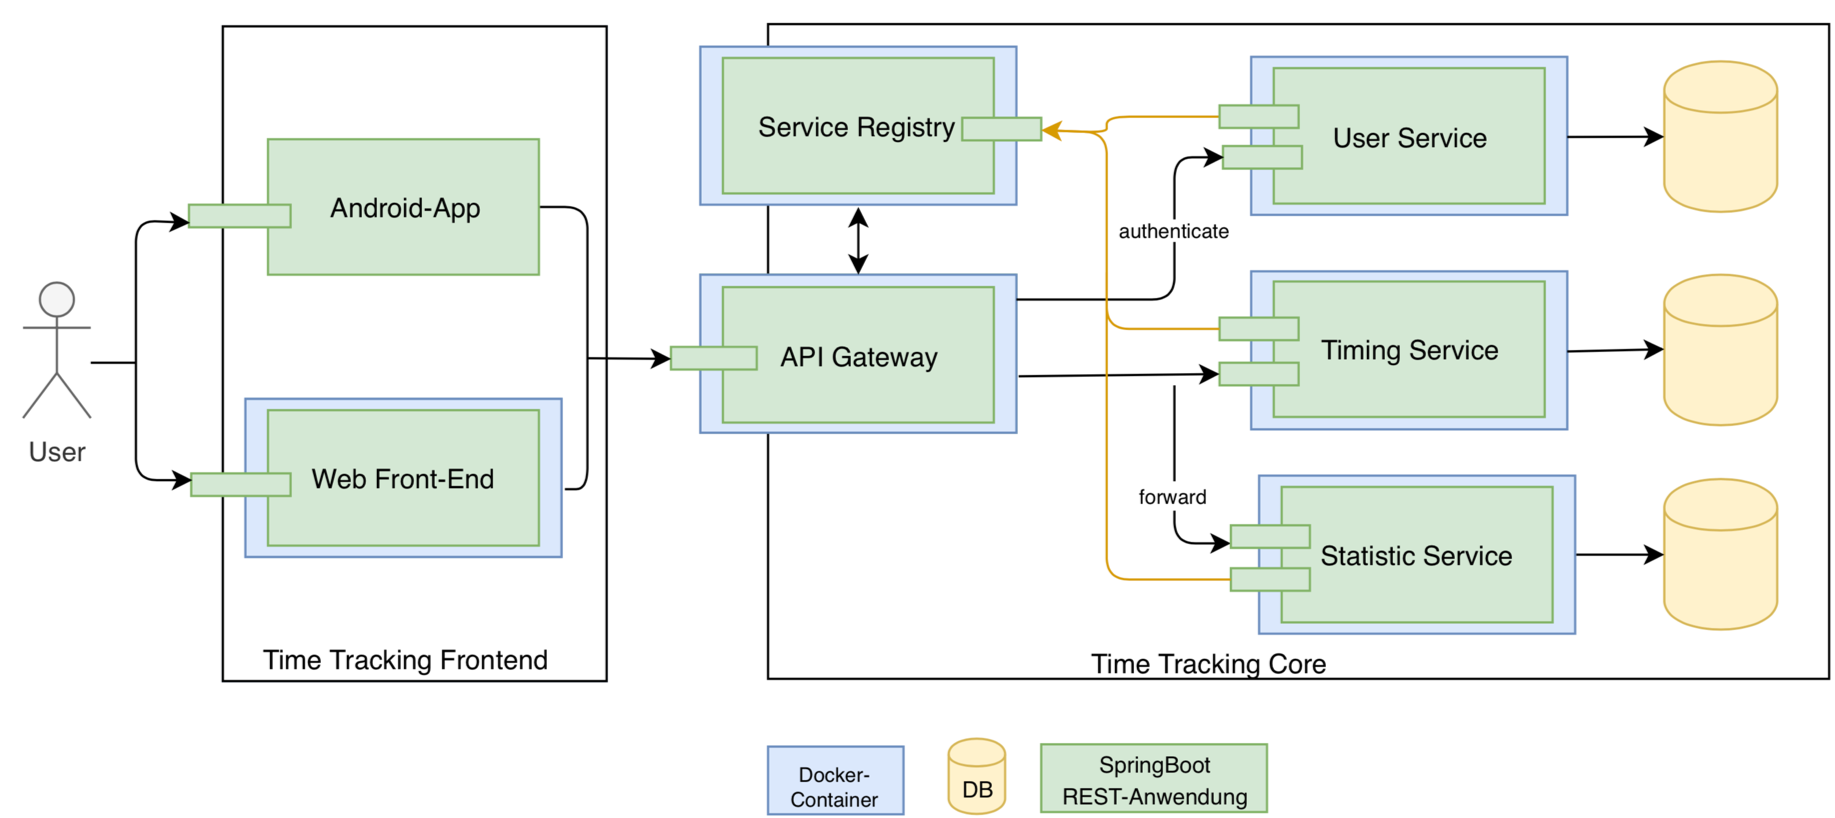
\includegraphics[width=1.15\linewidth]{SCC_Architecture-99final.png}
	\caption{Architektur von TimeTracker}
	\label{fig:Architektur}
\end{figure}



\begin{figure}[H]
	\hspace{-1.5cm}
	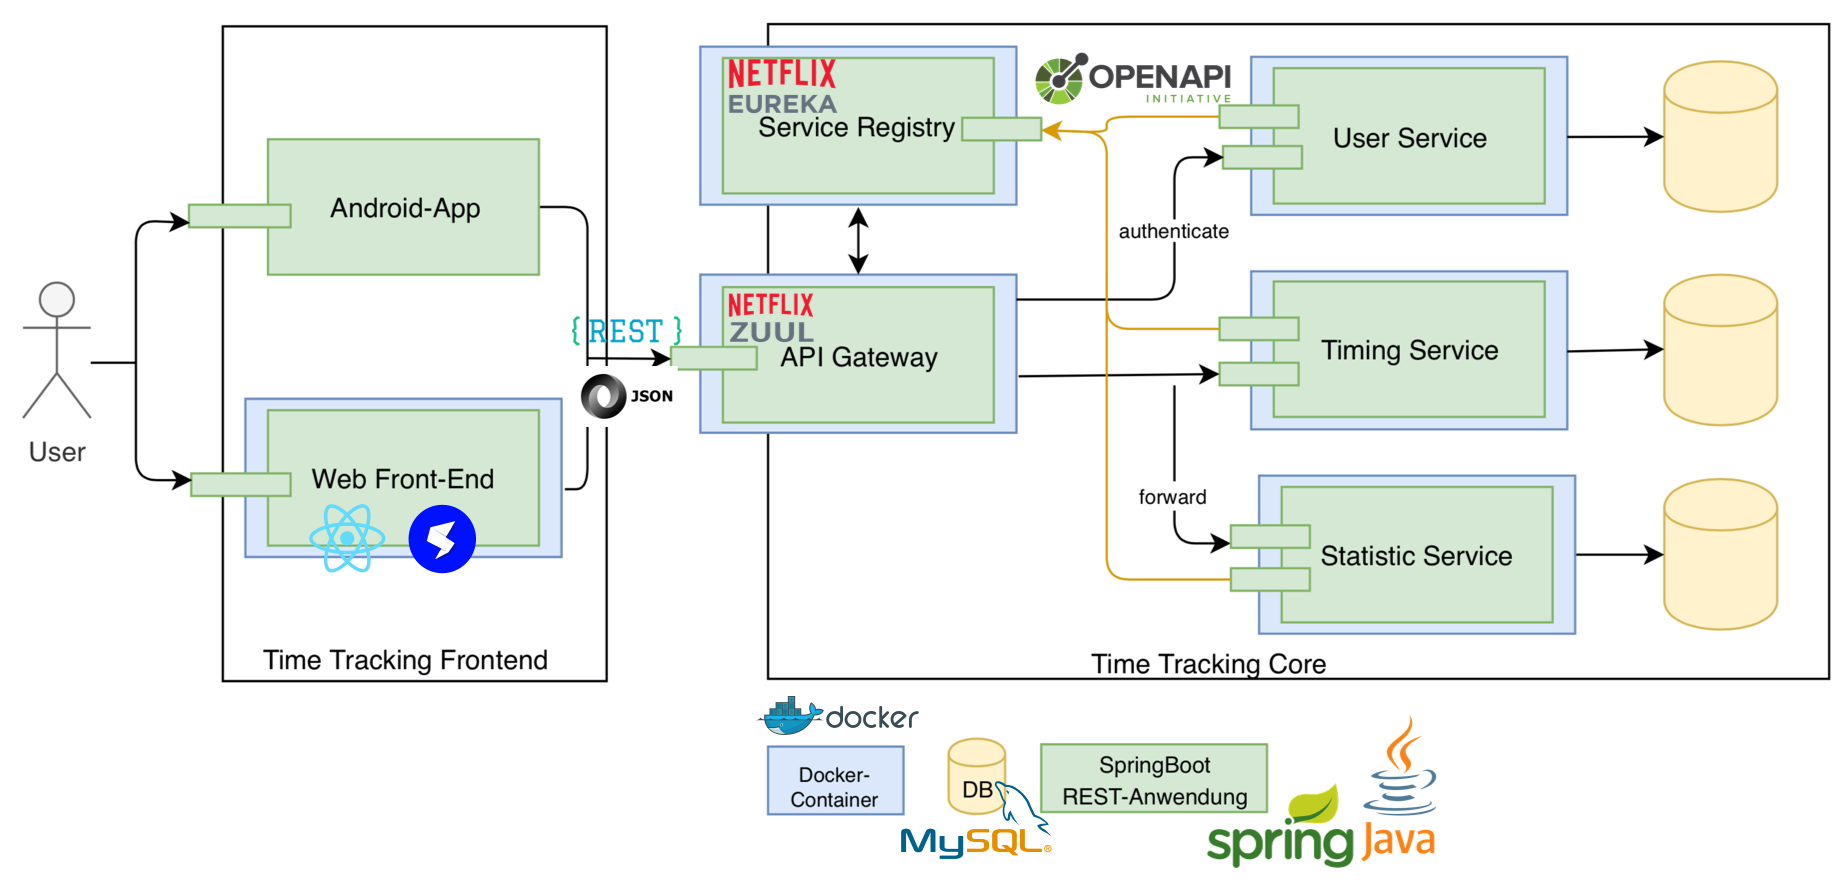
\includegraphics[width=1.15\linewidth]{SCC_Archtitecture_Technology.png}
	\caption{Architektur mit zugeordneten Technologien}
	\label{fig:ArchitekturTech}
\end{figure}





\paragraph{Funktionalität der Services}
\begin{itemize}
	\item User Service
	\begin{itemize}
		\item Registrierung
		\item Login
	\end{itemize}
	\item Timing Service
	\begin{itemize}
		\item Anlegen/ Abruf von Aktivitäten
		\item Anlegen/ Abruf von Records
		\item Abruf von Statistiken
	\end{itemize}
	\item Frontend Service
	\begin{itemize}
		\item Aufruf von UI
	\end{itemize}
	\item Service Registry
	\begin{itemize}
		\item Hält Services vor
	\end{itemize}
	\item API Gateway
	\begin{itemize}
		\item Nutzt Service Registry
		\item Mapping der Requests auf entsprechenden Service
	\end{itemize}
\end{itemize}

Die Dockerisierung und Nutzung von docker compose sowie docker stack ermöglicht das Ausrollen kontinuierlicher Updates.

\subsection{Schnittstellen}
% Links von Server mit http://editor.swagger.io/ oder https://swagger.io/tools/swagger-inspector/ or https://swagger.io/tools/swagger-ui/

Die API wurde mit Hilfe von OpenAPI und Swagger definiert und entwickelt. Mit Hilfe eines Swagger-Plugins für Maven wurden automatisch Java-Interfaces generiert, welche dann von Spring-Rest-Controllern implementiert werden konnten. Eine Auflistung aller Methoden ist über die folgenden Links zu erreichen. Zusätzlich befindet sich im Anhang (Seite \pageref{Anhang}) ein Ausdruck der automatisch generierten Dokumentation.

\begin{itemize}
	\item frontend-service: \newline  \url{https://app.swaggerhub.com/apis/SCC_Group4/frontend-service/}
	\item timing-service: \newline \url{https://app.swaggerhub.com/apis/SCC_Group4/timing-service/}
	\item user-service: \newline \url{https://app.swaggerhub.com/apis/SCC_Group4/user-service/}
\end{itemize}

\subsection{Sicherheit}

Die sichere und authentifizierte Kommunikation mit den Micro-Services wurde mit Hilfe von \textbf{JSON Web Token (JWT)} und HTTPS umgesetzt. Bei erfolgreichem Login erhält der Benutzer ein Token, mit dem er sich bei den Diensten authentifizieren kann.  Das Token wird im localStorage des Browsers gespeichert und bei jedem Request im Header mitgeführt. Dank Spring ist jedem Dienst dabei frei überlassen, wie das Token interpretiert wird, da ein entsprechendes Interface für jeden Service frei implementiert werden kann. So kann zum Beispiel Autorisierung auf Basis von Rollen realisiert werden. In unserer Anwendung findet dieses Feature jedoch keine Bedeutung, so dass jeder Micro-Service für sich nur die Validität des Tokens überprüft.

Des Weiteren wird die Sicherheit der Verbindung mittels der Transportverschlüsselung \textbf{HTTPS} gewährleistet.  Dazu wird im Produktionsbetrieb der gesamten Architektur ein nginx-Server vorgeschoben, der HTTPS-Requests entgegen nimmt, TLS-Termination vornimmt und die dann entschlüsselte Kommunikation an das API-Gateway weiterleitet. Die Kommunikation innerhalb des V-Servers, also zwischen den Micro-Services selbst, ist folglich weiterhin unverschlüsselt (HTTP). Wir haben uns bewusst dazu entschieden, da Verteilung von Zertifikaten sowie das ständige Ver- und Entschlüsseln der Kommunikation die Performance sichtlich beeinflusste.
